\csname documentclass\endcsname[../main.tex]{subfiles}
\usepackage[utf8x]{inputenc}
\usepackage{blindtext}
\usepackage{float}
\usepackage{graphicx}
\usepackage{siunitx}
\usepackage{cite}
\usepackage{hyperref}
\usepackage{cleveref}

\begin{document}

As stated earlier the predecessor to CLICK-B/C, CLICK-A, was responsible for demonstrating downlink capabilities using an optical terminal. 
The CLICK-B/C mission is responsible for showcasing both downlink and crosslink communications using an optical transceiver terminal \cite{click_b}.
The CLICK-B/C are identical 3U CubeSats supporting a laser communications terminal to demonstrate crosslink communication at distances of \(\qty{25}{\kilo\meter} - \qty{580}{\kilo\meter}\) with data rates \(\ge\qty[per-mode = symbol,per-symbol = p]{20}{\mega\bit\per\second}\).

\subsection{Concept of Operations (ConOps)}

The two CLICK-B/C spacecrafts are deployed in LEO within the same orbital plane, thus meaning, one leads the other follows.
The missions operation center will provide details on differential drag maneuvers via a S-band radio contact \cite{click_b_2}.
In order to realize each others position, the spacecrafts will be provided with ephemeris data by the mission operation center in hopes that a S-band crosslink is closed.
Once the crosslink closes, the on-board GPS exchanges navigation information which stays fresh for up to 2 minutes before time-out if closed-loop tracking isn't started \cite{click_b_2}.

\begin{figure*}[t]
    \centering
    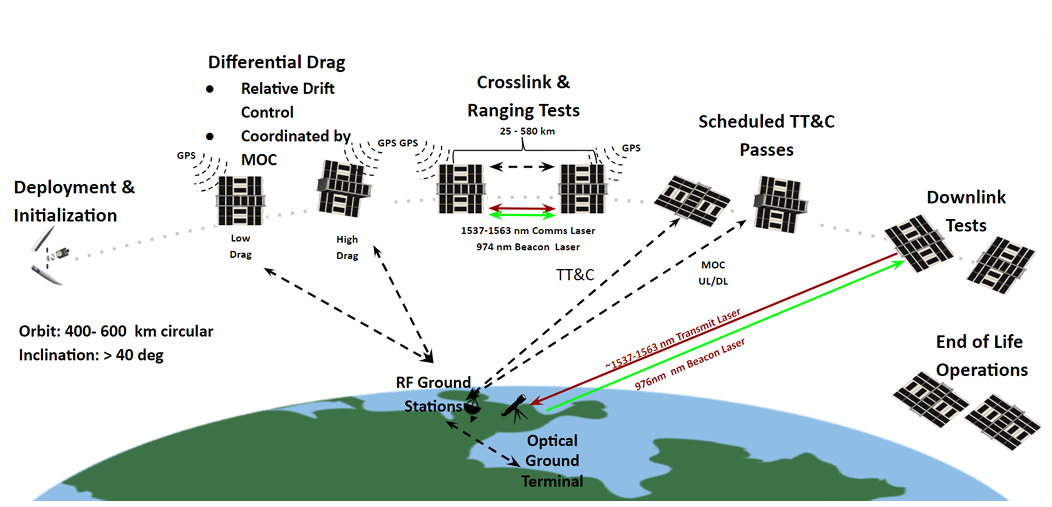
\includegraphics[width=\textwidth, height=200pt]{images/click_b_conops.PNG}
    \caption{Concept of Operations for the CLICK-B/C mission \cite{click_b}.}
    \label{fig:conops_b}
\end{figure*}

An overview of the ConOps for the CLICK-B/C mission is shown in \Cref{fig:conops_b}

\subsection{Link Budgets}

\Cref{fig:link_b} shows the Link Budget for the crosslink at, both, the maximum and minimum required ranges (\qty{25}{\kilo\meter} and \qty{580}{\kilo\meter}, respectively).
The terminal parameters determine the fixed parameters: the transmit power (\(P_{Tx}\)), transmit gain (\(G_{Tx}\)), receive gain (\(G_{Rx}\)), and the transmitter and receiver implementation losses (\(L_{Tx,imp}\) and \(L_{Rx,imp}\)).
The implementation losses are gathered from the optical coatings and the fiber losses, while the transmit gain and pointing loss is determined by the beam divergence.

Three link budgets have been created to design and approximate size of the optical systems for CLICK-B/C. Below covers the three links \cite{click_b}:
\begin{itemize}
    \item \textbf{Link 1:} the link between the transmit laser and the avalanche photodiode (APD) \cite{click_b}
    \item \textbf{Link 2:} the link between the beacon laser to the quadcell \cite{click_b}
    \item \textbf{Link 3:} the link between the beacon laser and the camera \cite{click_b}
\end{itemize}
The parameters, losses, and the Signal-to-Noise Ratio (SNR) for the various links can be found, once again, in \Cref{fig:link_b}. The figure also shows that in the case for the quadcell, the range variation plays little to no part in the pointing errors \cite{click_b_2}.

\begin{figure*}[t]
    \centering
    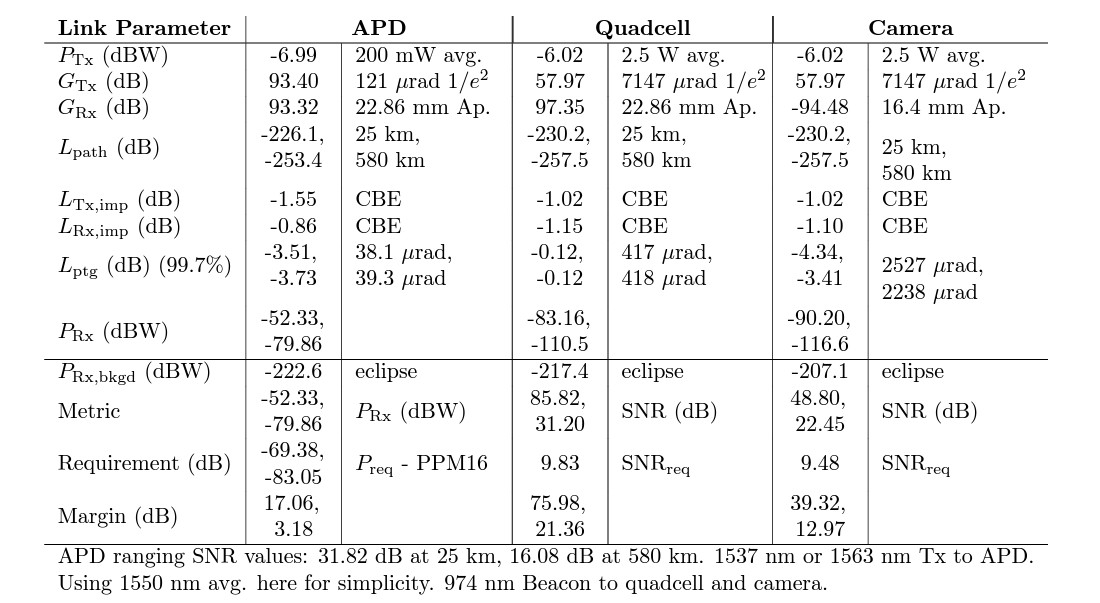
\includegraphics[width=\textwidth, height=300pt]{images/click_b_link.PNG}
    \caption{Concept of Operations for the CLICK-B/C mission \cite{click_b}.}
    \label{fig:link_b}
\end{figure*}


\end{document}